\documentclass[12pt,fleqn]{article}
\usepackage{xiiiemc}
\usepackage{natbib}
\usepackage{fancyhdr}
\usepackage{color}
\usepackage{wallpaper}
\usepackage{titlesec}   %% Define space between paragraph e section
\usepackage{float} 	%% Use to fix Figure or Table: ex: \begin{table}[H]
%%%%Don't edit this block. It reduces the spacing between the lines of the references
\let\OLDthebibliography\thebibliography
\renewcommand\thebibliography[1]{\OLDthebibliography{#1} \setlength{\parskip}{0pt}\setlength{\itemsep}{0pt plus 0.3ex}}



%%-----------------------------------------------EDIT-----------------------------------------------
\title{COMPARISON BETWEEN DIFFERENTIAL EVOLUTION AND SIMULATED ANNEALING ALGORITHMS APPLIED TO THE CONSTRUCTAL DESIGN OF DOUBLE-T SHAPED CAVITIES}

%%-----------------------------------------------EDIT----------------------------------------------
\author
    {\rm \begin{tabular}{l}
    \textbf{Gill Velleda Gonzales}$^{1,2}$ - {\textnormal gillgonzales@ifsul.edu.br}\\%
    \textbf{Elizaldo Domingues dos Santos}$^{2}$ - {\textnormal elizaldodossantos@gmail.com}\\
    \textbf{Antônio José da Silva Neto}$^{3}$ - {\textnormal ajsneto@iprj.uerj.br}\\
    \textbf{Liércio André Isoldi}$^{2}$ - {\textnormal liercioisoldi@gmail.com}\\
    \textbf{Luiz Alberto Oliveira Rocha}$^{2}$ - {\textnormal laorocha@gmail.com}\\
    {\fontsize{11}{0}\selectfont $^{1}$Instituto Federal Sul-Rio-Grandense - Campus Santana do Livramento, RS, Brazil}\vspace*{-0.05cm} \\
    {\fontsize{11}{0}\selectfont $^{2}$Universidade Federal do Rio Grande - PPG em Modelagem Computacional, Rio Grande, RS, Brazil}\vspace*{-0.05cm}\\
    {\fontsize{11}{0}\selectfont $^{3}$Universidade do Estado do Rio de Janeiro, Instituto Politécnico - Nova Friburgo, RJ, Brazil}
  \end{tabular}}
%%----------------------------------------------------------------------------------------------

\fancypagestyle{firspagetstyle}
{
	\lhead{}
	\fancyhead[C]{%
		
\includegraphics[width=0.75\linewidth]{logo}\\%
		{\scriptsize \fontfamily{phv}\fontseries{b}\selectfont \color[rgb]{0.45,0.45,0.45}
		08 a 11 de Outubro de 2018\\
		Instituto Federal Fluminense\\
		Búzios - RJ\\
	    }
	}
	\renewcommand{\headrulewidth}{0.0pt}
	\fancyfoot[C]{\footnotesize \parbox{15cm} {\centering  \fontsize{7.5}{0}\selectfont \it Anais do XXI ENMC – Encontro Nacional de Modelagem Computacional e IX ECTM – Encontro de Ciências e Tecnologia de Materiais,  Búzios, RJ – 08 a 11 Outubro 2018}} % \ttfamil
	\rhead{}
}

\newcommand\tab[1][0.75cm]{\hspace*{#1}}

\begin{document}
\maketitle

\thispagestyle{firspagetstyle}

\fancyhead[L]{\footnotesize{\fontsize{7.5}{0}\selectfont \it XXI ENMC e IX ECTM\\
	08 a 11 de Outubro de 2018\\
	Instituto Federal Fluminense – Búzios - RJ\\}}
\renewcommand{\headrulewidth}{0.0pt}
\fancyfoot[C]{\footnotesize \parbox{15cm} {\centering  \fontsize{7.5}{0}\selectfont \it Anais do XXI ENMC – Encontro Nacional de Modelagem Computacional e IX ECTM – Encontro de Ciências e Tecnologia de Materiais,  Búzios, RJ – 08 a 11 Outubro 2018}} % \ttfamil
\rhead{}

\begin{abstract}
In this paper, it is analyzed the application of two meta-heuristic methods, Differential Evolution and Simulated Annealing, for the geometric optimization of a complex cavity intruded into a heat conducting solid wall. The geometric evaluation is performed with Constructal Design method, which is used to define the performance parameter, constraints and degrees of freedom of the problem to be optimized. The main purpose of this work is the comparison between the results of this two meta-heuristics, mainly for reproduction of the effect of degrees of freedom over the thermal performance of the studied problem. The experiment consists on the simulation of thirty runs for each algorithm, with different values for the configuration parameters, and also four versions of Differential Evolution and five versions of Simulated Annealing. The optimization results show that the meta-heuristic algorithm and its parameter configuration is important for proper prediction of the effect of degrees of freedom over the thermal performance and definition of system design. Results also indicated that one of the Differential evolution algorithms led to the best and most robust performance. Therefore, the significant contribution here is the recommendation of the more reliable meta-heuristic, and its correct parameters for the studied problem.
\end{abstract}

\keywords{\em{Heat Transfer, Constructal Design, Simulated Annealing, Differential Evolution, Geometric Optimization }}

\pagestyle{fancy}

\section{INTRODUCTION}
The geometric optimization of cooling cavities inside a solid with heat generation using Constructal Design for geometric evaluation was first proposed by \cite{Biserni2004}. In this study, C and T-shaped cavities were investigated.Constructal Design is a method used to prove that the design of all flow systems of finite dimensions can be predicted by a physical principle named Constructal Law \citep{Bejan}. This principle determines the shapes and structures that emerge in nature. The Constructal Law explains that for a finite-size flow system to persist in time (to survive) its configuration must evolve in such a way that it provides easier access to the currents that flow through it \citep{Bejan}. The CD method is not an optimization method but a method for geometrical evaluation based on performance indicators and constraints (physical, geometrical). More precisely, the method has been used to definition of search space, which must be investigated with an optimization method, e.g., Exhaustive Search (ES).  In this method, all geometric possibilities are evaluated considering an increment of variation of the geometric parameters. However, its employment becomes prohibitive for complex shapes (with several degrees of freedom) due to high computational effort \cite{Gonzales2015a}.

After the pioneer work of Biserni et al. (2004), more complex shapes were investigated using CD associated with ES. For instance, \citep{Biserni2007} studied H-shaped cavities and \citep{Lorenzini2011} investigated Y-shaped ones. The comparison between different shapes of cavities, kepting the same constraints, has indicated that as more complex is the cavity shape the best is the thermal performance of the system (for systems with high intensity). Examples of this behavior can be seen in recent studies of complex and several cavities \citep{Xie2010,Lorenzini2012,Lorenzini2014}. However, complex cavities need more degrees of freedom and require more computational effort in the optimization process. Therefore, for complex cavities, meta-heuristic methods have been used as alternative for geometrical evaluation, allowing the study of many degrees of freedom. \cite{Lorenzini2014} used Genetic Algorithm (GA) to optimize a complex Y-shaped cavity considering the effect of a convective parameter over the problem design. The GA was also associated with CD for geometric optimization of morphing fins coupled with a trapezoidal heat generating body in the study of \cite{Biserni2017}. \cite{Gonzales2015a} analyzed the performance of different parameters of Simulated Annealing (SA) algorithm in the geometric optimization of a Y-shaped cavity. The work of \cite{Gonzales2015a} compared various parameters of the Cooling Schedule (CS) for SA algorithm. It was noticed that a hybrid parameters led to the best thermal performances and improve the representation of the geometric parameters effect over thermal performance of the studied problem. Recently, \cite{Gonzales2017} performed a comparison between the Luus-Jaakola and SA algorithms with hybrid parameters of CS applied in the Double-T shaped cavity optimization. Results showed that the best performance was reached with the SA algorithm with hybrid parameter for Cooling Schedule.

In the present work, the meta-heuristic of SA is compared with the Differential Evolution (DE) algorithm to the geometric optimization of the Double-T shaped cavity. The main purpose of the system is to minimize the maximal excess of temperature in the solid domain. The Double-T Shaped cavity was first proposed by \cite{Gonzales2015b}, and the SA was used in the geometric optimization. The two algorithms are performed with distinct parameters, and then the comparison is made between the variations of SA and DE. The best versions for each meta-heuristic are then compared. The SA variations differ in the Cooling Schedule (CS) parameter, and five distinct CS are investigated. Different versions of the DE algorithm are also compared. The DE variations differ in the crossover and mutation operators, and four DE algorithms are performed. The double-T shaped cavity has five degrees of freedom (DOFs) that define the cavity geometry ($H/L$, $H_{0}/L_{0}$, $H_{1}/L_{1}$, $H_{2}/L_{2}$ and $S_{1}/H_{0}$). Four and five DOFs are optimized, and each algorithm achieves the curve of the effect of DOF over optimal geometry and thermal performance. The results for each algorithm are registered in a database and analyzed. Therefore, the comparison between the results of the algorithms is performed through the effect of DOF over optimal geometry, not only using the minimal maximum excess of temperature.  Then, it is evaluated here the algorithm that is more able to reproduce the effect of the degrees of freedom over the performance of the system.

\section{MATHEMATICAL AND NUMERICAL MODEL}


Figure \ref{figure01} shows the heat transfer problem of interest, that consists in a conducting body in the two-dimensional configuration, with the third dimension, with length $W$, perpendicular to the plane of the figure. The solid domain has a constant and uniform internal heat generation with the volumetric rate given by $q^{'''}(Wm^{\tiny -3})$. The solid has a constant thermal conductivity k. The outer surfaces of the solid are perfectly insulated, corresponding to adiabatic conditions. In this case, the heat can only be removed through the double-T shaped cavity, which is kept at a minimum temperature $(\theta_{min})$. The minimal temperature of the cavity may be kept with the flow of refrigerant fluid through the cavity, changing phase at a low temperature. For the sake of simplicity, the heat transfer coefficient on the cavity wall is assumed to be sufficiently large so that the convective resistance can be neglected in comparison to the solid conduction resistance.

\begin{figure}[H]
\centering
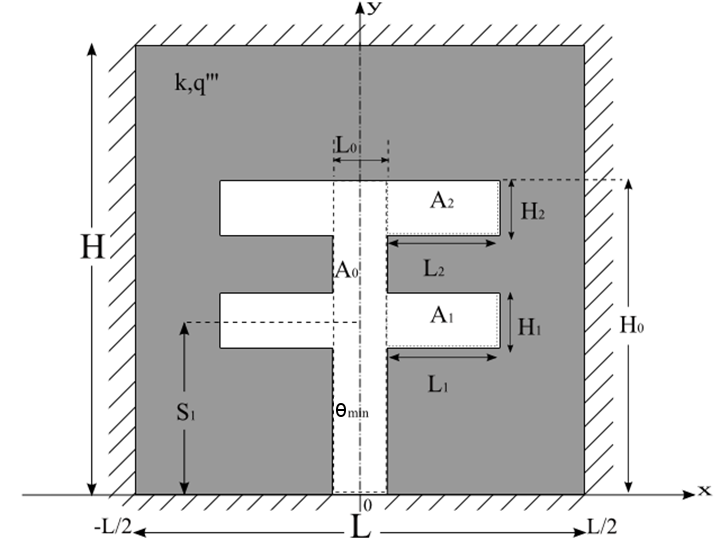
\includegraphics[width=0.6\linewidth]{imgs/duplo_t.png}
\caption{ {\small Computational domain of Double-T shaped cavity.}}
\label{figure01}
\end{figure}

The objective of the analysis is to determine the optimal geometry ($H/L$, $H_{0}/L_{0}$, $H_{1}/L_{1}$, $H_{2}/L_{2}$ and $S_{1}/H_{0}$) that is characterized by the minimum global thermal resistance $(\theta_{max} - \theta_{min})/(q^{'''}A)$. According to the CD the geometric evaluation can be subjected to total and cavity areas constraints, represented respectively by:

\begin{equation}
A = HL \label{area_total}
\end{equation}
\begin{equation}
A_{c} = A_{0} + 2A_{1} + 2A_{2} \label{area_cavidade}
\end{equation}
\tab The fraction of the cavity area with respect to the total area is given by:
\begin{equation}
\phi_{c} = A_{c}/A \label{fi}
\end{equation}
\tab For the determination of the temperature field in the solid domain, it is necessary to solve the heat conduction equation given by:
\begin{equation}
\frac{\partial^{2} \theta}{\partial \tilde{x}^{2}}+\frac{\partial^{2} \theta}{\partial \tilde{y}^{2}}+1=0\label{calor}
\end{equation}

For the sake of brevity, the equations with dimensionless variables, the equations of boundary conditions of minimum temperature are not reproduced here. More details can be seen in the work of \cite{Gonzales2015b}. The aim is to minimize the maximal excess temperature represented by the following equation:

\begin{equation}
\tilde{\theta}_{max}=\frac{\theta_{max}-\theta_{min}}{q^{'''}\cdot\frac{A}{k}}\label{fo}
\end{equation}

The determination of $\tilde{\theta}_{max}$ is needed to optimize the five degrees of freedom ($H/L$, $H_{0}/L_{0}$, $H_{1}/L_{1}$, $H_{2}/L_{2}$ and $S_{1}/H_{0}$) submitted to the corresponding constraints of the cavity area ($\phi_{c}$, $\phi_{1}$ and $\phi_{2}$) and the total solid area. Where $\phi_{1}$ and $\phi_{2}$ represent the dimensionless area of each branch of the Double-T shaped cavity. In this paper are optimized the five DOFs ($H/L$, $H_{0}/L_{0}$, $H_{1}/L_{1}$, $H_{2}/L_{2}$ and $S_{1}/H_{0}$). The function represented by Eq. (\ref{fo}) is determined numerically by solving Eq. (\ref{calor}) for the temperature field in every assumed configuration ($H/L$, $H_{0}/L_{0}$, $H_{1}/L_{1}$, $H_{2}/L_{2}$ and $S_{1}/H_{0}$), and calculating $\tilde{\theta}_{max}$ to see whether its value may be minimized by varying the configuration. The numerical solution is performed with the Finite Element Method (FEM)\citep{Reddy1994}, based on linear triangular elements, available in the The MATLAB$^{\tiny ®}$ environment, with the PDE (partial-differential-equations) toolbox. The grid was non-uniform in both x and y directions, and varied from one geometry to the next. The appropriate mesh size was determined by successive refinements (h-adaptively), increasing the number of elements four times from one current mesh size to the next one. For the sake of brevity, the grid independence test can be seen in \cite{Gonzales2015b}, and, therefore, it is note repeated.

\section{GEOMETRIC OPTIMIZATION}

The CD method is employed to determine the values for the  objectives and constraints chosen, as well as, the search space and the degrees of freedom (DOFs). With the optimization problem defined, the search for the optimal geometry was performed with two optimization algorithms, SA and DE. The parameters of these two heuristic methods applied are also investigated. Therefore, the results are compared in order to indicate the best method for the problem evaluated here. The SA algorithm, proposed by \cite{Kirkpatrick1983}, has as main parameter the function that controls the temperature decay, named Cooling Schedule. Five different functions of Cooling Schedules (CS) are tested in this study, the traditional schedules Boltz and Exponential, implemented in the MATLAB$^{\tiny ®}$ optimization toolbox, and named here respectively as SAEX and SABO. Also hybrid CS are investigates (BoltzExp, ConstExp1, and ConstExp2) proposed by \cite{Gonzaes2015a, Gonzales2015b}, named respectively as SABE, SAC1 and SAC2. The DE is an evolutionary-based algorithm proposed by \cite{Storn1997} for continuous spaces. In this work, the DE algorithm is also varied in four versions, two versions with basic DE strategy for mutation operator named DE/rand/1/bin and two version with the DE/best/2/bin variant of mutation operator \citep{Storn1997}. The algorithm named DE1 and DE2 are variant of basic DE strategy and the versions named here as DE3 and DE4 have the approach of  DE/best/2/bin. The DE heuristic have more two parameters varied in this paper, the Crossover (CR) rate and the factor $F$, which controls the amplification of differential variation. The DE1 and DE4 have the factor $F=1.5$ and $CR=0.7$, while the DE2 and DE3 versions has factor $F=2$ and $CR=0.9$.

The geometric optimization of double-T shaped cavity is realized by the variation of the parameters that define its geometry and, according to the CD method, this process must be submitted to constraints. The cavity studied here has nine variables ($H$, $L$, $H_{0}$, $L_{0}$, $H_{1}$, $L_{1}$, $H_{2}$, $L_{2}$ and $S1$) and four constraints ($A$, $\phi_{c}$, $\phi_{1}$ and $\phi_{2}$). Then, five degrees of freedom are required to closure the equation system which defines the geometry ($H/L$, $H_{0}/L_{0}$, $H_{1}/L_{1}$, $H_{2}/L_{2}$ and $S_{1}/H_{0}$). The optimization process is concentrated in four and five DOFs since these conditions represent the most critical situation of evaluation. Firstly, the four DOFs optimization is performed by the optimization of the three DOFs ( $H_{1}/L_{1}$, $H_{2}/L_{2}$ and $S_{1}/H_{0}$) for ten different values of $H_{0}/L_{0}$,  keeping fixed  H/L = 1 and the four study constraints are kept as $A$ = 1, $\phi_{c}$ = 0.1; $\phi_{1}$ = 0.015; and $\phi_{2}$ = 0.015. The five DOFs optimization is performed by the optimization of four DOFs ($H_{0}/L_{0}$, $H_{1}/L_{1}$, $H_{2}/L_{2}$ and $S_{1}/H_{0}$) for ten different values of H/L.  The constraints are kept with the same values used in the four  DOFs optimization. Therefore, at the end of the four  DOFs optimization process, each algorithm conducts to results of the effect of the ratio $H_{0}/L_{0}$ over the four times minimized maximal excess of temperature, $({\theta}_{max})_{3\times m}$, and their respective optimal shapes. The curve of effect of the DOF $H/L$ over optimal geometry, is also obtained in the five DOFs optimization process. More details about the definition of geometric variables as function of restrictions and degrees of freedom can be seen in \cite{Gonzales2015b}.

\section{RESULTS AND DISCUSSIONS}

The results of the four DOFs optimization process performed by thirty runs of each algorithm, with different versions of SA and DE algorithms, were achieved and saved in a database. The algorithms have the number of iterations limited to 150. All the algorithms conduct to the optimal geometry and maximum excess of temperature three times minimized. However, because of the stochastic nature, the algorithms do not produce the same results in all thirty rounds, and the average value is obtained to construct the results seen in Fig. \ref{figure02}, allowing to observe the algorithm version that is closer to the benchmark solution (reached with Exhaustive Search).


In the Figure \ref{figure02} (a), it is possible observe the effect of $H_{0}/L_{0}$ over $({\theta}_{max})_{3\times m}$ obtained with all algorithms. It can be observed that all methods led to similar results for $H_{0}/L_{0}=10$. For ratios $H_{0}/L_{0}>10$ same differences are noticed. The results reached with DE algorithms have the best agreement with the benchmark solution, mainly the DE1 version. In spite of some differences, results reached with this version properly reproduced the effect of $H_{0}/L_{0}$ over $({\theta}_{max})_{3\times m}$. The SA versions with the cooling schedule functions Exponential (SAEX), Boltzmann (SABO) and hybrid BoltExp (SABE) led to the worst performance for reproduction of the effect of  $H_{0}/L_{0}$ over $({\theta}_{max})_{3\times m}$.

Figure \ref{figure02}(b) shows the results of each algorithm analysed in this paper for the effect of  $H_{0}/L_{0}$ over $H_{2}/L_{2}$ three times optimized, $(H_{2}/L_{2})_{3\times o}$. A similar tendency observed in the effect of of $H_{0}/L_{0}$ over $({\theta}_{max})_{3\times m}$ is reached for the effect of $H_{0}/L_{0}$ over the $(H_{2}/L_{2})_{3\times o}$. The best agreements where found for $H_{0}/L_{0}<=10$, with exception of SA Exponential where poor agreement is found. For $H_{0}/L_{0}>10$ the best representation of the effect of $H_{0}/L_{0}$ over $(H_{2}/L_{2})_{3\times o}$ is obtained with DE1 and DE3. Some discrepancies are seen for the highest magnitudes of $H_{0}/L_{0}$, probably by the found of some local optimal shapes.

The effect of $H_{0}/L_{0}$ over $(H_{1}/L_{1})_{2\times o}$ and $(S_{1}/H_{0})_{o}$ is showed in the Fig. \ref{figure03}(a) and Fig. \ref{figure03}(b), respectively. The curvature represented by the black line in the \ref{figure03} (a) and (b) reproduce the effect of $H_{0}/L_{0}$ over the optimal values of the DOFs investigated. Other curves represent mean values obtained with each algorithm. In the Fig. \ref{figure03}(a) results of all algorithms show a large discrepancy between optimal values of $(H_{1}/L_{1})_{2\times o}$ achieved with SA and DE methods studied here for $H_{0}/L_{0}<10$. For $H_{0}/L_{0}>10$ the averages reached with all algorithm converges to correct magnitudes.It is worth to emphasize that differences seen for $H_{0}/L_{0}<10$ do not affected the global performance due to the insensitivity of this degree of freedom over the thermal performance. except for the SA algorithm with Exponential cooling schedule (SAEX). In the Figure \ref{figure03}(b) the effect of $H_{0}/L_{0}$ over $(S_{1}/H_{0})_{o}$ was better reproduced by the versions of DE algorithm and two versions of SA algorithm (sac1 and sac2). The DE1 and DE2 algorithms achieved the best predictions among the compared algorithms.

\begin{figure}[H]
\centering
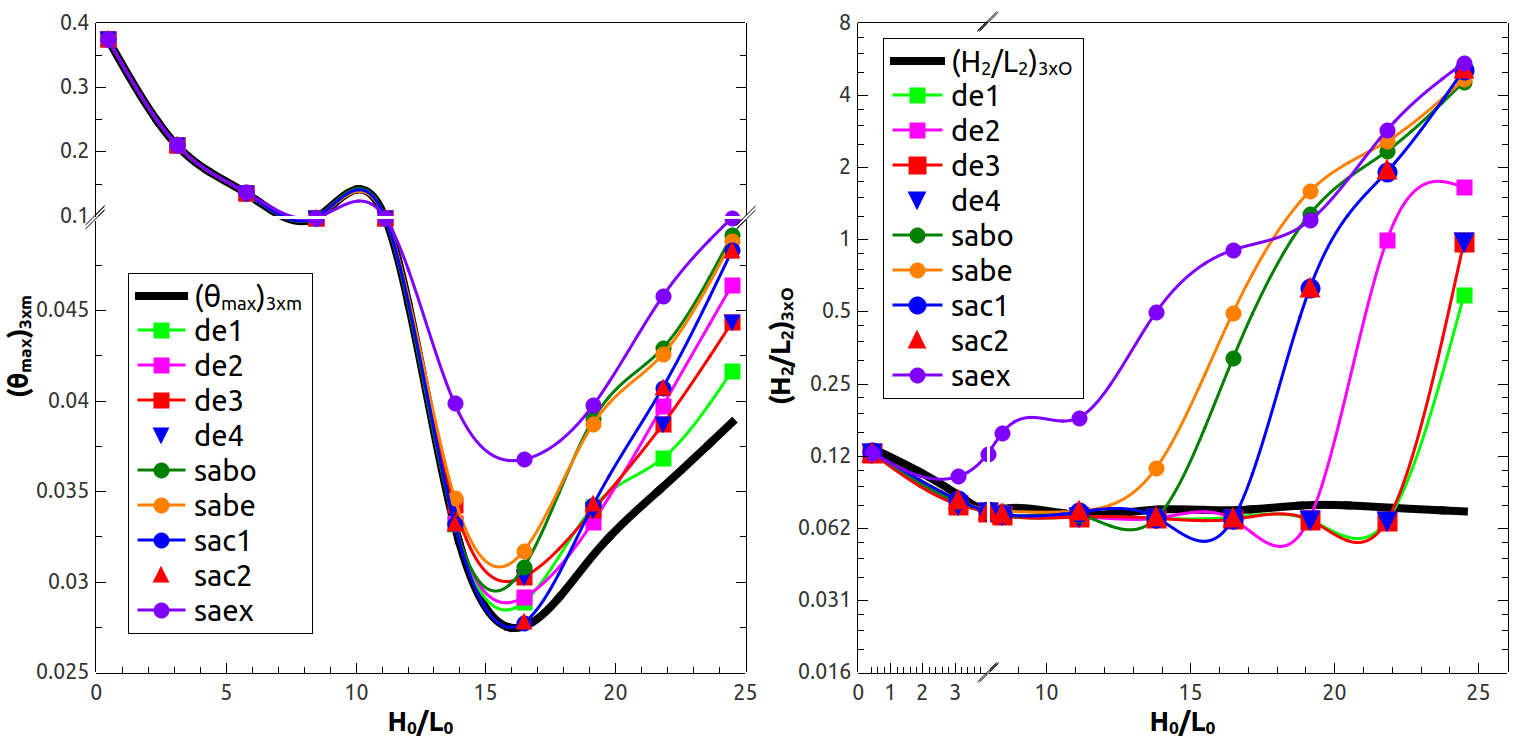
\includegraphics[width=0.8\linewidth]{imgs/4dof/de_sa_h0l0-tmin-4dof.png}
\caption{ {\small Effect of $H_{0}/L_{0}$ over $({\theta}_{max})_{3\times m}$ and $(H_{2}/L_{2})_{3\times o}$ obtained with different DE and SA algorithms over:  a) over $({\theta}_{max})_{3\times m}$. b) over $(H_{2}/L_{2})_{3\times o}$ }}
\label{figure02}
\end{figure}

\begin{figure}[H]
\centering
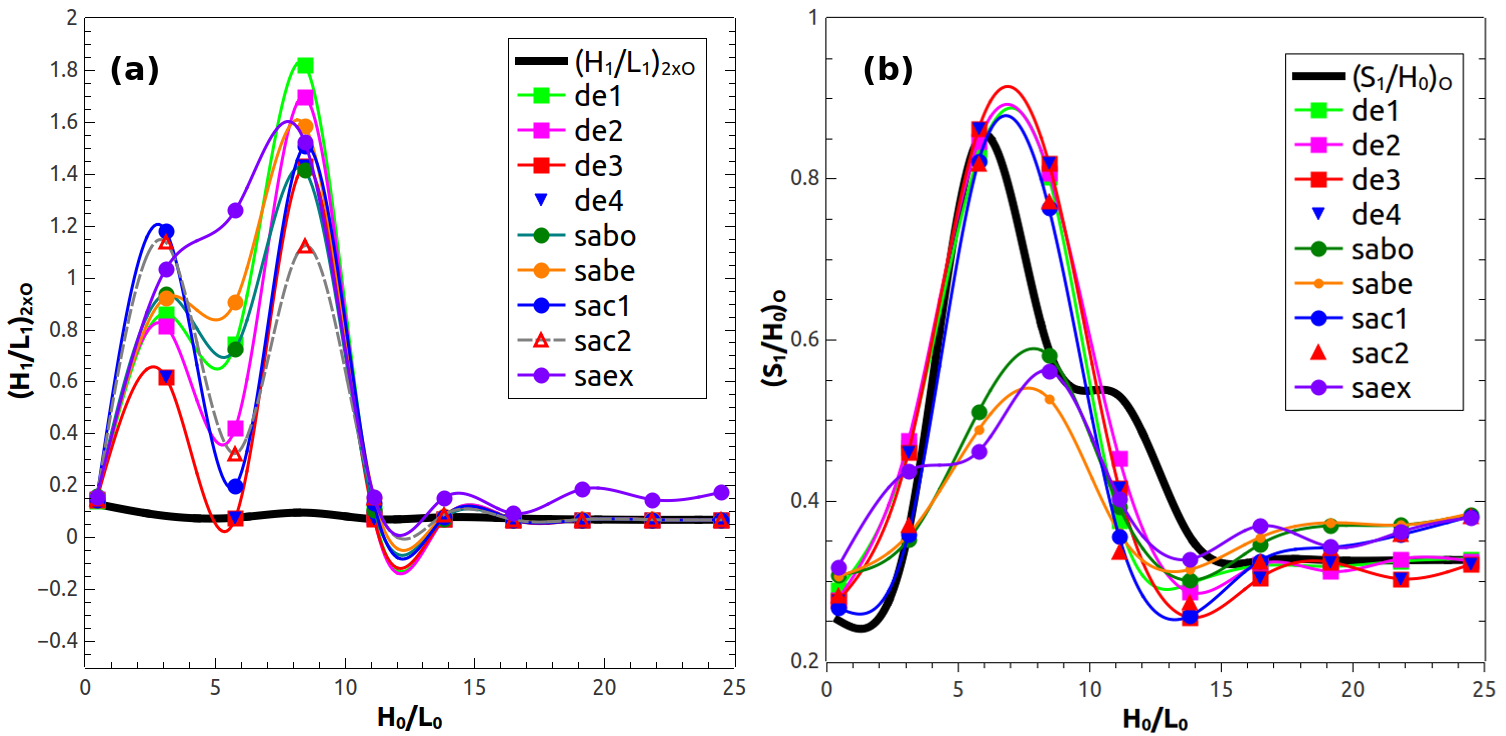
\includegraphics[width=0.8\linewidth]{imgs/4dof/de_sa_h0l0-h1l1-s1h0-4dof.png}
\caption{ {\small Effect of $H_{0}/L_{0}$ over $(H_{1}/L_{1})_{2\times o}$ and $(S_{1}/H_{0})_{o}$ obtained with different DE and SA algorithms over: a) $(H_{1}/L_{1})_{2\times o}$, b) $(S_{1}/H_{0})_{o}$ }}
\label{figure03}
\end{figure}

For the evaluation of 5 DOFs, the number of iterations was changed to 300 in order to improve the seek for the effect of $H/L$ over the thermal performance and optimal shapes. For each ratio of $H/L$ 30 runs of each algorithm were performed and the maximum excess of temperature four times minimized are recorded for different magnitudes of $H/L$ studied here. Then, it is possible to reproduce the effect of $H/L$ over $({\theta}_{max})_{4\times m}$ and respective optimal shapes. Statistical measures were also stored in a database, as well as, the minimal values of the maximum excess of temperature four times minimized and its respective optimal geometries.

Figure \ref{figure04} shows  the minimal values of the maximum excess of temperature four times minimized represented by the black line, and other curves represent the average of this value reached for each algorithm in the geometric optimization process of five DOFs ($H/L$, $H_{0}/L_{0}$, $H_{1}/L_{1}$, $H_{2}/L_{2}$ and $S_{1}/H_{0}$). Results of Fig. 4(a) and 4(b) show that the effect of $H/L$ over $({\theta}_{max})_{4\times m}$ is better reproduced with DE algorithm versions than SA ones. For values of $H/L > 0.5$ all algorithms can reproduce the effect of $H/L$ of $({\theta}_{max})_{4\times m}$ with precision. The same behavior was observed for degree of freedom $(H_{0}/L_{0})$, where all algorithms can predict the effect of $H/L$ over ${(H_{0}/L_{0})_{4\times o}}$.



Figure \ref{figure06} shows the comparison between the results of the versions of DE algorithm and variants of the SA algorithm to predict effect of $H/L$ over ${(H_{2}/L_{2})_{3\times o}}$. In this case,variations of DE algorithm have a good agreement with benchmark solution, with exception of DE2 version which showed some oscillations for $H/L< 0.5$. The results of the SA algorithm, Fig. \ref{figure06}(b), show some differences for $H/L < 5.0$ in spite of representation of a similar tendency. For the lowest values of ratio $H/L$, none of SA algorithms reproduced the magnitudes of ${(H_{2}/L_{2})_{3\times o}}$. For values of $H/L > 5$ the versions of SA algorithm SAC1 and SAC2 achieved the most similar magnitudes in comparison with ${(H_{2}/L_{2})_{3\times o}}$. The difficulty of the versions of SA algorithm to reach the optimal configuration of $H_{2}/L_{2}$ for the lowest magnitudes of $H/L$ explain the differences found for $({\theta}_{max})_{4\times m}$ showed in the Fig.\ref{figure04}(b).

\begin{figure}[H]
\centering
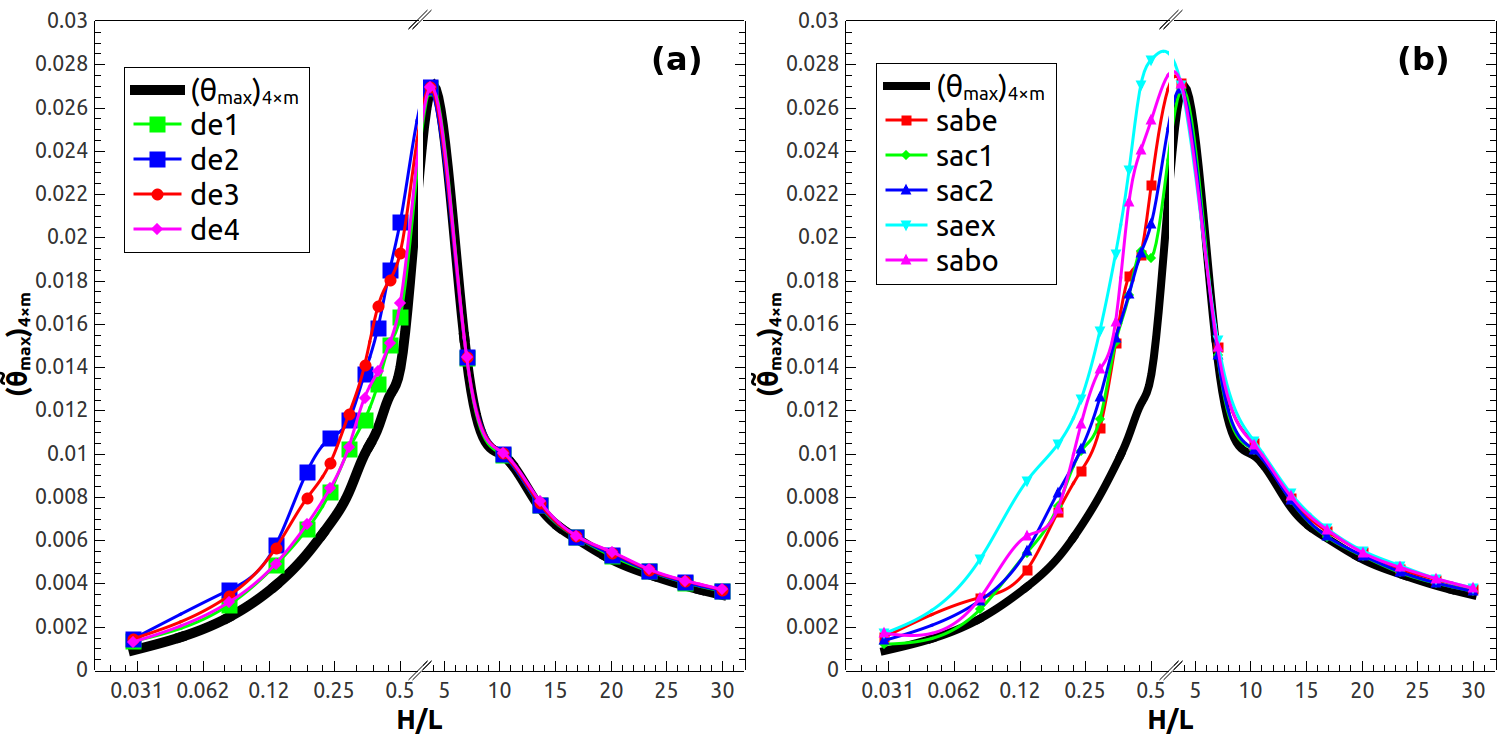
\includegraphics[width=0.9\linewidth]{imgs/5dof/de_sa_hl_tmin.png}
\caption{ {\small Effect of $H/L$ over $({\theta}_{max})_{4\times m}$ obtained by different optimization methods: a) DE algorithm, b) SA algorithm}}
\label{figure04}
\end{figure}

\begin{figure}[H]
\centering
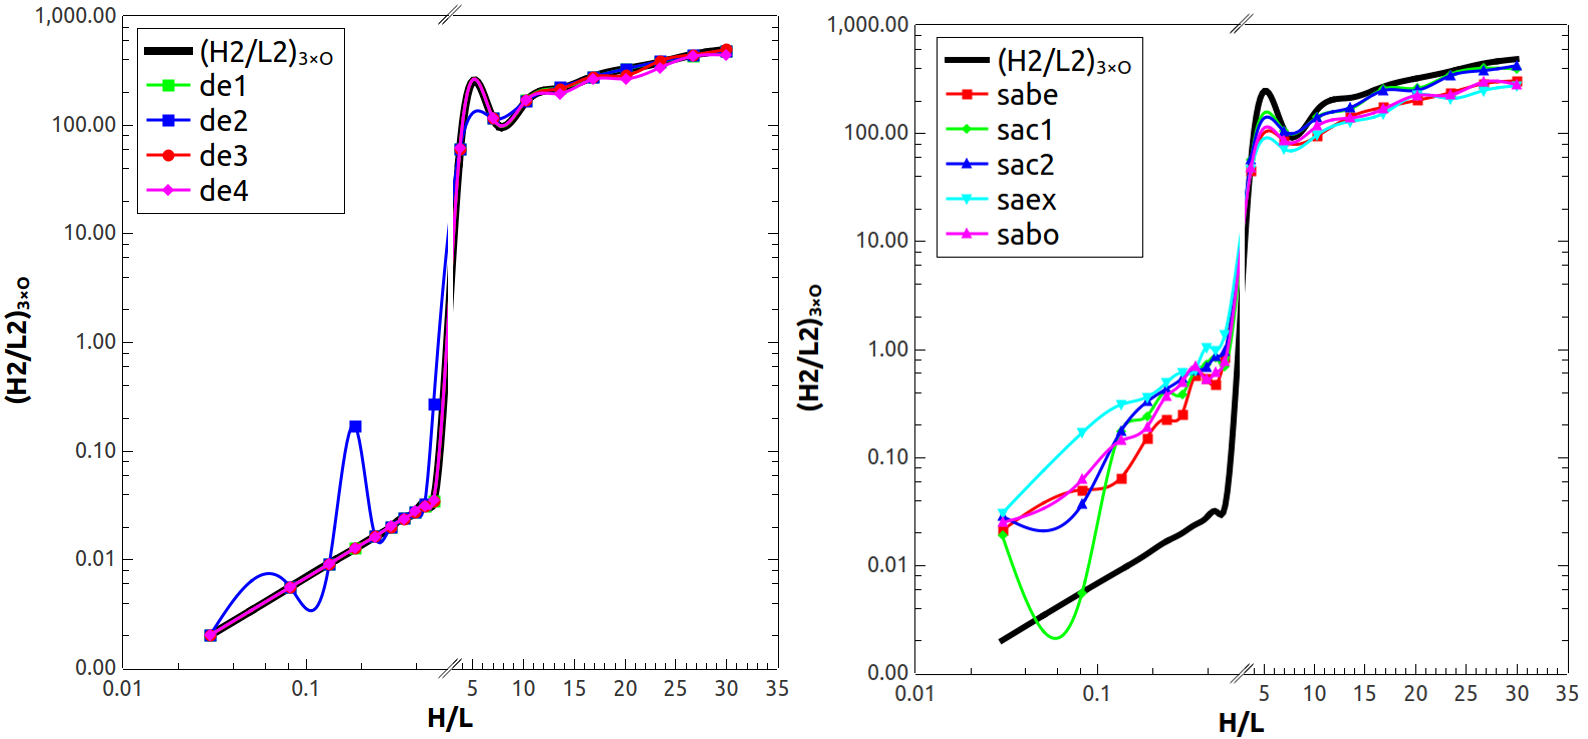
\includegraphics[width=0.9\linewidth]{imgs/5dof/de_sa_hl_h2l2.png}
\caption{ {\small Effect of $H/L$ over ${(H_{2}/L_{2})_{3\times o}}$ obtained by different optimization methods: a) DE algorithm, b) SA algorithm}}
\label{figure06}
\end{figure}


The effect of $H/L$ over ${(H_{1}/L_{1})_{2\times o}}$ is shown in the Figure \ref{figure07}. Fig. \ref{figure07}(a) shows the results of DE algorithms while Fig. \ref{figure07}(b) illustrate the results achieved with SA algorithms. As can be seen, results reached with DE led to a closer concordance with benchmark solution than those reached with SA. Among the DE algorithms, the best results are obtained with DE1 and DE2. The versions of the SA algorithm achieve divergent results for this DOF, where the worst performance is reached with SAEX, followed by  SABE and SABO. The other versions (SAC1 and SAC2) are more similar to those reached with DE3 and DE4 for higher magnitudes of $H/L$.


\begin{figure}[H]
\centering
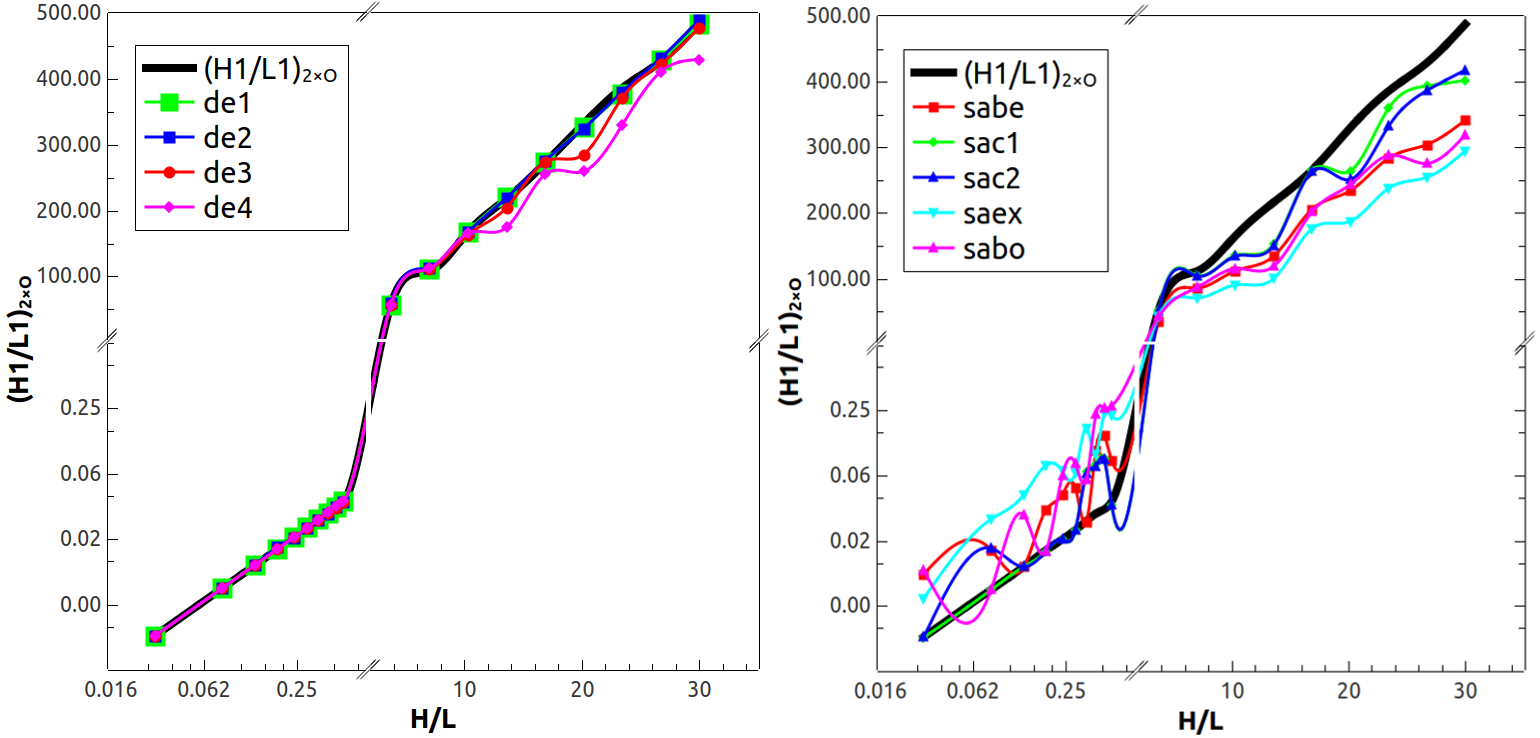
\includegraphics[width=0.9\linewidth]{imgs/5dof/de_sa_hl_h1l1.png}
\caption{ {\small Effect of $H/L$ over ${(H_{1}/L_{1})_{2\times o}}$ obtained by different optimization methods: a) DE algorithm, b) SA algorithm}}
\label{figure07}
\end{figure}

In Figure \ref{figure08}, it is possible to note that the results of all algorithms diverge from the optimal values of ${(S_{1}/H_{0})_{2\times o}}$ for all ratios of $H/L$. The results in Fig \ref{figure08}(a) shows that all versions of DE algorithm do not reach the optimal values of ${(S_{1}/H_{0})_{2\times o}}$ for lower ratios of  $H/L$. In spite of this fact, DE1 results have a similar tendency to that predicted with benchmark solution. The Fig. \ref{figure08}(b) shows that versions of SA algorithm have a high difficult to represent the optimal values of ${(S_{1}/H_{0})_{2\times o}}$ for any ratio of  $H/L$ analyzed.
\begin{figure}[H]
\centering
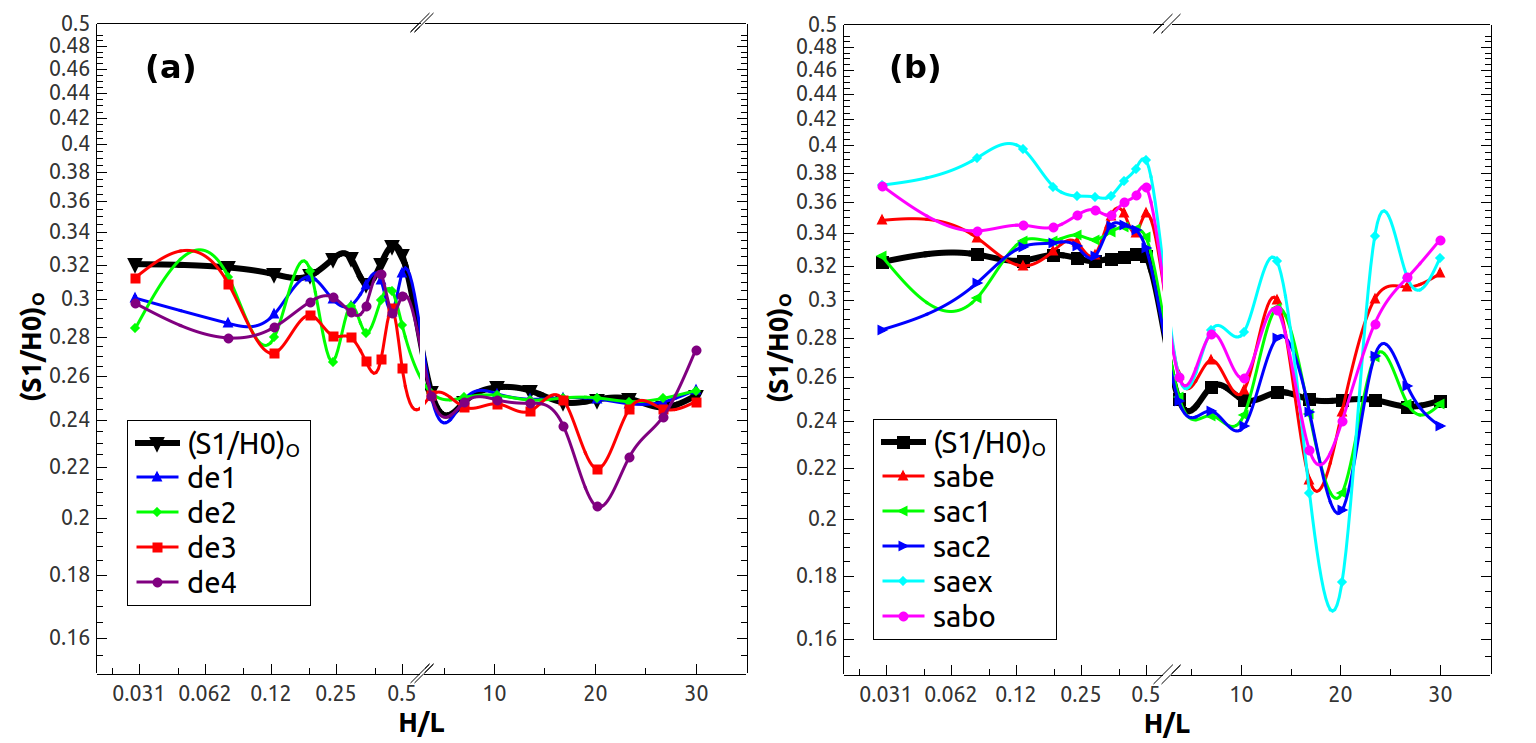
\includegraphics[width=0.9\linewidth]{imgs/5dof/de_sa_hl_s1h0.png}
\caption{ {\small Effect of $H/L$ over ${(S_{1}/H_{0})_{O}}$ obtained by different optimization methods: a) DE algorithm, b) SA algorithm}}
\label{figure08}
\end{figure}

\section{CONCLUSIONS}

The present work studied the employment of two meta-heuristic, Simulated Annealing (SA) and Differential Evolution (DE), combined with Constructal Design (CD) to perform a geometric optimization in a heat transfer problem. The problem consists of a cooled double-T shaped cavity intruded into a conductive solid wall with constant heat generation. The geometric optimization problem is conducted by the CD method that defines the Degrees of Freedom (DOFs) and constraints. The purpose is to compare the results of the two heuristics to evaluate the efficiency to reproduce the effect of geometric parameters over four and five times minimized maximal excess of temperature reached in the solid wall and respective optimal configurations for degrees of freedom. The evaluation of geometric configurations over the flow system performance is an important subject into Constructal Design framework. Then, the present study aimed to contribute with recommendations about the best optimization methods to be associated with Constructal Design to reproduction of geometry effect over system performance.

The SA algorithm versions led to inferior performance than that reached with DE methods. However, in an inner comparison between SA versions, the best performance was achieved with hybrid functions of Cooling Schedules (CS) in agreement with previous founds of \cite{Gonzales2015a,Gonzales2015b}.

Results of optimization for four degrees of freedom indicated that DE algorithms were succesfull for reproduction of the effect of degrees of freedom over thermal performance in most of the investigations performed, mainly the DE1 version. For the geometric optimization of five DOF, the versions of DE algorithm also were superior to the results of SA algorithm. For the evaluation with 5 degrees of freedom, the DE1 version again was the most well succeded to find the best shapes. Results also showed that the DE2 algorithm achieved good results for some cases, as the effect of $H/L$ over ${(S_{1}/H_{0})_{O}}$ and over ${(H_{1}/L_{1})_{2  \times o}}$. However, this version of DE algorithm led to worst results on the effect of $H/L$ over ${(H_{1}/L_{1})_{2  \times o}}$ which influenced the results of $({\theta}_{max})_{4\times m}$. Differences in the Crossover rate ($CR$) and amplification factor ($F$) can explain the differences found for two versions of DE (DE1 and DE2). Probably, the parameters used for DE2 does not represent adequate values to be employed for the present problem. An example is that the DE3 also have the worst results compared to the DE4 version of DE algorithm, and it have the same parameters of $CR$ and $F$ that DE2. Therefore, it is possible to conclude that, for the studied problem, DE algorithm with parameters used in DE1 are the best recommendation for optimization of cavity problems, mainly for reproduction of the effect of DOFs over thermal performance and other degrees of freedom.




\subsection*{\textit{Acknowledgements}}
G. V. Gonzales acknowledges IF-SUL and PPGMC-FURG by support. E. D. dos Santos is sponsored by CNPq (Process: 306024/2017-9). Antônio J. Silva Neto acknowledges the financial support provided by FAPERJ, CNPq and CAPES.


% ------------------------------------------------------------------------

\fontsize{11}{0}\selectfont
\bibliographystyle{xiiiemc}
\bibliography{bibfile}
% ------------------------------------------------------------------------

%For papers written in Portuguese or Spanish.

%\begin{center}
%  TITLE IN ENGLISH
%\end{center}

%\def\abstractname{Abstract}%

%\begin{abstract}
%   Abstract in english
%\end{abstract}

%\keywords{\em{Keywords in english}}

\end{document}
